\chapter{USRP}
\section{Introduction}

The USRP (Universal Software Radio Peripheral) is intended to provide a low-cost, high quality hardware platform for software radio. It is designed and marketed by Ettus Research, LLC. It is commonly used by research labs, universities, and hobbyists. The USRP platform is designed for RF applications from DC to 6 GHz. USRPs connect to a host computer through a high-speed USB or Gigabit Ethernet link, which the host-based software uses to control the USRP hardware and transmit/receive data.

The USRP Hardware Driver (UHD) is the official driver for all Ettus Research products. The UHD supports Linux, Mac OS X and Windows.

\begin{figure}[h]
\centering
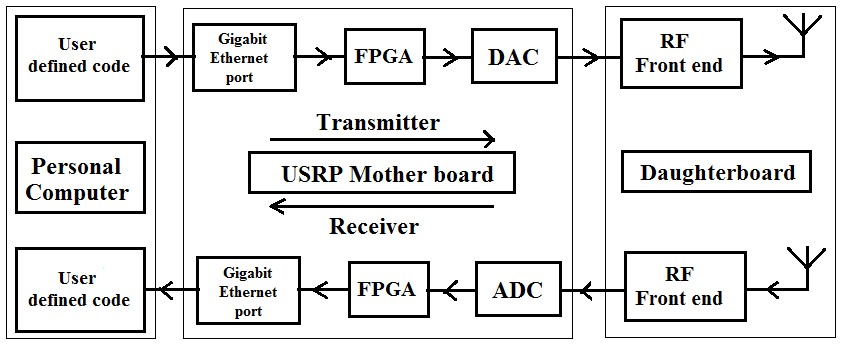
\includegraphics[width=0.8\textwidth]{usrpBlock}
\caption[Block diagram of USRP]{Block diagram of USRP. \emph{Source:  Kranthi Ananthula, Experimental setup of Cognitive Radio Test-Bed using Software Defined Radio , M. Tech Dissertation , 2013.}}
\label{usrpBlock}
\end{figure}

In this project we are using a particular model of USRP product known as the USRP N210.

\section{USRP N210}

The USRP N200 and N210 are the highest performing class of hardware of the USRP family of products, which enables engineers to rapidly design and implement powerful, flexible software radio systems. The N200 and N210 hardware is ideally suited for applications requiring high RF performance and great bandwidth. Such applications include physical layer prototyping, dynamic spectrum access and cognitive radio, spectrum monitoring, record and playback, and even networked sensor deployment.
The Networked Series products offers MIMO capability with high bandwidth and dynamic range. The Gigabit Ethernet interface serves as the connection between the N200/N210 and the host computer. This enables the user to realize 50 MS/s of real-time bandwidth in the receive and transmit directions, simultaneously (full duplex).

